\chapter{Exercise Types}\label{s:exercises}

\begin{objectives}

\item Describe four types of formative assessment exercises for
  programming classes.

\item Describe two kinds of feedback on programming exercises that can
  be given by automated tools.

\end{objectives}

Every good carpenter has a set of screwdrivers, and every good teacher
has different kinds of formative assessment exercises to check what
learners are actually learning, help them practice their new skills,
and keep them engaged.  This chapter starts by describing several
kinds of exercises you can use to check if your teaching has been
effective.  It then looks at the state of the art in automated
grading, and closes by exploring discussion, projects, and other
important kinds of work that require more human attention to assess.
Our discussion draws in part on the
\href{http://web-cat.org/questionbank/}{Canterbury Question Bank}
\cite{Sand2013}, which has entries for various languages and topics in
introductory computing.

\section{The Classics}\label{s:exercises-classics}

As \secref{s:models-formative-assessment} discussed, \emph{multiple
  choice questions} (MCQs) are most effective when the wrong answers
probe for specific misconceptions.  In terms of Bloom's Taxonomy
(\secref{s:process-objectives}), MCQs are usually designed to test
recall and understanding (``What is the capital of Saskatchewan?''),
but they can also require learners to exercise judgment.

\begin{callout}{A Multiple Choice Question}

  In what order do operations occur when the computer evaluates the
  expression \texttt{price~=~addTaxes(cost~-~discount)}?

  \noindent
  a) subtraction, function call, assignment \\
  b) function call, subtraction, assignment \\
  c) function call, then assignment and subtraction simultaneously \\
  d) none of the above

\end{callout}

The second classic type of programming exercise is \emph{code and run}
(C\&R), in which the learner writes code that produces a specified
output.  C\&R exercises can be as simple or as complex as the teacher
wants, but for in-class use, they should be brief and have only one or
two plausible correct answers. For novices, it's often enough to ask
them to call a specific function: experienced teachers often forget
how hard it can be to figure out which parameters go where.  For more
advanced learners, figuring out which function to call is more
engaging and a better gauge of their understanding.

\begin{callout}{Code \& Run}

  The variable \texttt{picture} contains a full-color image read from
  a file.  Using one function, create a black and white version of the
  image and assign it to a new variable called \texttt{monochrome}.

\end{callout}

\noindent
Write and run exercises can be combined with MCQs.  For example, this
MCQ can only be answered by running the Unix \texttt{ls} command:

\begin{callout}{Combining MCQ with Code \& Run}

  You are in the directory \texttt{/home/greg}. Which of the following
  files is \emph{not} in that directory?

  \noindent
  a) \texttt{autumn.csv} \\
  b) \texttt{fall.csv} \\
  c) \texttt{spring.csv} \\
  d) \texttt{winter.csv}

\end{callout}

C\&Rs help learners practice the skills they most want to learn, but
they can be hard to assess: learners can find lots of unexpected ways
to get the right answer, and are demoralized if an automatic grading
system rejects their code because it doesn't match the instructor's.
One way to reduce how often this occurs is to assess only their
output, but that doesn't give them feedback on how they are
programming.  Another is to give them a small test suite they can run
their code against before they submit it (at which point it is run
against a more comprehensive set of tests). Doing this helps them
figure out if they have completely misunderstood the intent of the
exercise before they do anything that they think might cost them
grades.

Instead of writing code that satisfies some specification, learners
can be asked to write tests to determine whether a piece of code
conforms to a spec.  This is a useful skill in its own right, and
doing it may give students a bit more sympathy for how hard their
teachers work.

\begin{callout}{Inverting Code \& Run}

  The function \texttt{monotonic\_sum} calculates the sum of each
  section of a list of numbers in which the values are strictly
  increasing. For example, given the input
  \texttt{{[}1, 3, 3, 4, 5, 1{]}}, the output is
  \texttt{{[}4, 12, 1{]}}. Write and run unit tests to determine
  which of the following bugs the function contains:

  \begin{itemize}
  \item
    Considers every negative number the start of a new sub-sequence.
  \item
    Does not include the first value of each sub-sequence in the
    sub-sum.
  \item
    Does not include the last value of each sub-sequence in the
    sub-sum.
  \item
    Only re-starts the sum when values decrease rather than fail to
    increase.
\end{itemize}

\end{callout}

\emph{Fill in the blanks} is a refinement of C\&R in which the learner
is given some starter code and has to complete it. (In practice, most
C\&R exercises are actually fill in the blanks because the teacher
will provide comments to remind the learners of the steps they should
take.) As discussed in \chapref{s:load}, novices often find filling in
the blanks less intimidating than writing all the code from scratch,
and since the teacher has provided most of the answer's structure,
submissions are much more predictable and therefore easier to check.

\begin{callout}{Fill in the Blanks}

  Fill in the blanks so that the code below prints the string
  \texttt{'hat'}.

\begin{verbatim}
text = 'all that it is'
slice = text[____:____]
print(slice)
\end{verbatim}

\end{callout}

As described in \chapref{s:load}, \glossref{g:parsons-problem}{Parsons
  Problems} also avoid the ``blank screen of terror'' problem.  The
learner is given the lines of code needed to solve a problem, but has
to put them in the right order. Research over the past few years has
shown that Parsons Problems are effective because they allow learners
to concentrate on control flow separately from vocabulary
\cite{Pars2006,Eric2015,Morr2016,Eric2017}. The same research shows
that giving the learner more lines than she needs, or asking her to
rearrange some lines and add a few more, makes this kind of problem
significantly harder \cite{Harm2016}.  Tools for building and doing
Parsons Problems online exist \cite{Ihan2011}, but they can be
emulated (albeit somewhat clumsily) by asking learners to rearrange
lines of code in an editor.

\begin{callout}{Parsons Problem}

  Rearrange and indent these lines to sum the positive values in a
  list.  (You will need to add colons in appropriate places as well.)

\begin{verbatim}
total = 0
if v > 0
total += v
for v in values
\end{verbatim}

\end{callout}

\section{Tracing}\label{s:exercises-tracing}

\emph{Tracing execution} is the inverse of a Parsons Problem: given a
few lines of code, the learner has to trace the order in which those
lines are executed. This is an essential debugging skill, and is a
good way to solidify learners' understanding of loops, conditionals,
and the evaluation order of function and method calls. The easiest way
to implement it is to have learners write out a sequence of labelled
steps.  Having them choose the correct sequence from a set (i.e.,
presenting this as an MCQ) adds cognitive load without adding value,
since they have to do all the work of figuring out the correct
sequence, then search for it in the list of options.

\begin{callout}{Tracing Execution Order}

  In what order are the labelled lines in this block of code executed?

\begin{verbatim}
A)     vals = [-1, 0, 1]
B)     inverse_sum = 0
       try:
           for v in vals:
C)             inverse_sum += 1/v
       except:
D)         pass
\end{verbatim}

\end{callout}

\emph{Tracing values} is similar to tracing execution, but instead of
spelling out the order in which code is executed, the learner has to
list the values that one or more variables take on as the program
runs. It can also be implemented by having learners provide a list of
values, but another approach is to give the learner a table whose
columns are labelled with variable names and whose rows are labelled
with line numbers, and asking them to fill in all of the values taken
on by all of the variables.

\begin{callout}{Tracing Values}

  What values do \texttt{left} and \texttt{right} take on as this
  program executes?

\begin{verbatim}
left = 24
right = 6
while right:
    left, right = right, left % right
\end{verbatim}

\end{callout}

You can also require learners to trace code backwards, e.g., to figure
out what the input must have been if the code produced a particular
result \cite{Armo2008}.  These \emph{reverse execution} problems
require search and deductive reasoning, but they are particularly
useful when the ``output'' is an error message, and help learners
develop valuable debugging skills.

\begin{callout}{Reverse Execution}

  Fill in the missing number in \texttt{values} that caused this
  function to crash.

\begin{verbatim}
values = [ [1.0, -0.5], [3.0, 1.5], [2.5, ___] ]
runningTotal = 0.0
for (reading, scaling) in values:
    runningTotal += reading / scaling
\end{verbatim}
  
\end{callout}

\emph{Minimal fix} exercises also help learners develop debugging
skills.  Given a few lines of code that contain a bug, the learner
must either make or identify the smallest change that will produce the
correct output. Making the change can be done using C\&R, while
identifying it can be done as a multiple choice question.

\begin{callout}{Minimal Fix}

  This function is supposed to test whether a number lies within a
  range.  Make one small change so that it actually does so.

\begin{verbatim}
def inside(point, lower, higher):
    if (point <= lower):
        return false
    elif (point <= higher):
        return false
    else:
        return true
\end{verbatim}

\end{callout}

\emph{Theme and variation} exercises are similar, but instead of
making a change to fix a bug, the learner is asked to make a small
alteration that changes the output in some specific way.  Allowed
changes can include replacing one function call with another, changing
one variable's initial value, swapping an inner and outer loop,
changing the order of tests in a chain of conditionals, or changing
the nesting of function calls or the order in which methods are
chained.  Again, this kind of exercise gives learners a chance to
practice a useful real-world skill: the fastest way to produce a
working program is often to tweak one that already does something
useful.

\begin{callout}{Theme and Variations}

  Change the inner loop in the function below so that it fill the
  upper left triangle of an image with a specified color.

\begin{verbatim}
function fillTriangle(picture, color) is
    for x := 1 to picture.width do
        for y := 1 to picture.height do
            picture[x, y] = color
        end
    end
end
\end{verbatim}

\end{callout}

\emph{Refactoring exercises} are the complement of theme and variation
exercises: given a working piece of code, the learner has to modify it
in some way \emph{without} changing its output. For example, the
learner could be asked to replace loops with vectorized expressions,
to simplify the condition in a while loop, etc. The exercise here is
that there are often so many ways to refactor a piece of code that
grading requires human intervention.

\begin{callout}{Refactoring}

  Write a single list comprehension that has the same effect as this
  loop.

\begin{verbatim}
result = []
for v in values:
    if len(v) > threshold:
        result.append(v)
\end{verbatim}

\end{callout}

\section{Diagrams}\label{s:exercises-diagrams}

Having students draw concept maps and other diagrams gives insight
into how they're thinking (\secref{s:memory-concept-maps}), but
free-form diagrams take human time and judgment to assess.
\emph{Labelling diagrams}, on the other hand, is almost as useful from
a pedagogical point of view but much easier to scale.

Rather than having learners create diagrams from scratch, provide them
with a diagram and a set of labels and have them put the latter in the
right places on the former.  The diagram can be a complex data
structure (``after this code is executed, which variables point to
which parts of this structure?''), the graph that a program produces
(``match each of these pieces of code with the part of the graph it
generated''), the code itself (``match each term to an example of that
program element''), or many other things; the key is that constraining
the set of solutions makes this usable in class and at scale.

\begin{callout}{Labelling a Diagram}

  The tree below shows how a small fragment of HTML is represented in
  memory.  Put the labels 1--10 on the elements of the tree to show
  the order in which they are reached in a depth-first traversal.

  {\centering
    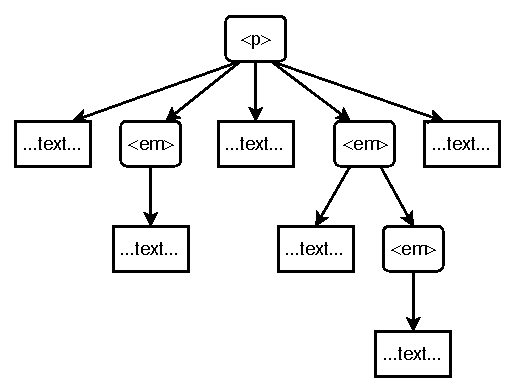
\includegraphics{../docs/fig/labelling.pdf}
  }

\end{callout}

Another way to use diagrams for formative assessment is to give
learners the pieces of the diagram and ask them to arrange them
correctly.  This is a visual equivalent of a Parsons Problem, and you
can provide as much or as little of a skeleton to help them with
placement as you think they're ready for.  (I have fond memories
of trying to place resistors and capacitors in a circuit diagram
in order to get the right voltage at a certain point, and have often
seen teachers give learners a fixed set of Scratch blocks and ask them
to create a particular drawing using only those blocks.)

\emph{Matching problems} can be thought of as a special case of
labelling in which the ``diagram'' is a column of text and the labels
are taken from the other column.  \emph{One-to-one matching} gives the
learner two lists of equal length and asks her to pair corresponding
items, e.g., ``match each piece of code with the output it produces''.

\begin{callout}{Matching}

  Match each regular expression operator with what it does.

  \begin{tabular}{ll}
    \texttt{?} & start of line \\
    \texttt{*} & zero or one occurrences \\
    \texttt{+} & end of line \\
    \texttt{\$} & one or more occurrences \\
    \texttt{\textasciicircum} & zero or more occurrences \\
  \end{tabular}

\end{callout}

\emph{Many-to-many matching} is similar, but the lists aren't the same
length, so some items may be matched to several others, while others
may not be matched at all. Both kinds require learners to use
higher-order thinking skills, but many-to-many are more difficult
because learners can't do easy matches first to reduce their search
space (i.e., there is a higher cognitive load.)

Matching problems can be implemented by having learners submit lists
of matching pairs as text (such as ``A3, B1, C2''), but that's clumsy
and error-prone.  Having them recognize a set of correct pairs in an
MCQ is even worse, as it's painfully easy to misread.

\emph{Ranking} is a special case of matching that is (slightly) more
amenable to answering via lists, since our minds are pretty good at
detecting errors or anomalies in sequences.  Give the learner several
items and ask them to order them from fastest to slowest, most robust
to most brittle, and so on.  The former tends toward recall (e.g.,
recognizing the names of various sorting algorithms and knowing their
properties), while the latter tends more toward reasoning and
judgment.

\emph{Summarization} also requires learners to use higher-order
thinking, and gives them a chance to practice a skill that is very
useful when reporting bugs rather than fixing them. For example,
learners can be asked, ``Which sentence best describes how the output
of f changes as x varies from 0 to 10?'' and then given several
options as a multiple choice question.

You can also ask for very short free-form answers to questions in
constrained domains, e.g., ``What is the key feature of a stable
sorting algorithm?''  We still can't fully automate checks for these
without a frustrating number of false positives (accepting wrong
answers) and false negatives (rejecting correct ones), but they lend
themselves well to peer grading (\secref{s:individual-peer}).

\section{Automatic Grading}\label{s:exercises-grading}

Automatic program grading tools have been around longer than I've been
alive: the earliest published mention dates from 1960 \cite{Holl1960},
and the surveys published in \cite{Douc2005,Ihan2010} mention many
specific tools by name.  Building such tools is a lot more complex
than it might first seem.  How are assignments represented? How are
submissions tracked and reported?  Can learners co-operate?  How can
submissions be executed safely? \cite{Edwa2014a} is an entire paper
devoted to an adaptive scheme for detecting and managing infinite
loops and other non-terminating code submissions, and that's just one
of the many issues that comes up.

As elsewhere, it's important to distinguish learner satisfaction from
learning outcomes.  \cite{Magu2018} switched informal programming labs
to a weekly machine-evaluated test for a second-year CS course using
an auto-grading tool originally developed for programming
competitions.  Learners didn't like the automated system, but the
overall failure rate for the course was halved, and the number of
learners gaining first class honors tripled.  In contrast,
\cite{Rubi2014} also began to use an auto-grader designed for
competitions, but saw no significant decrease in their learners'
dropout rates; once again, learners made some negative comments about
the tool, which the authors attribute to its feedback messages rather
than to dislike of auto-grading.

\cite{Srid2016} took a different approach.  They used
\glossref{g:fuzz-testing}{fuzz testing} (i.e., randomly-generated test
cases) to check whether learner code does the same thing as a
reference implementation supplied by the teacher.  In the first
project of a 1400-learner introductory course, fuzz testing caught
errors that were missed by a suite of hand-written test cases for more
than 48\% of learners, which clearly demonstrates its value.

\cite{Basu2015} gave learners a suite of solution test cases, but
learners had to unlock each one by answering questions about its
expected behavior before they were allowed to apply it to their
proposed solution.  For example, suppose learners are writing a
function to find the largest adjacent pair of numbers in a list;
before being allowed to use the tests associated with this question,
they have to choose the right answer to, ``What does
\texttt{largestPair(4, 3, -1, 5, 3, 3)} produce?''  (The correct
answer is \texttt{(5, 3)}.)  In a 1300-person university course, the
vast majority of learners chose to validate their understanding of
test cases this way before attempting to solve problems, and then
asked fewer questions and expressed less confusion about assignments.

It's common and tempting to use off-the-shelf style checking tools to
grade learners' code.  However, \cite{Nutb2016} initially found no
correlation between human-provided marks and style-checker rule
violations.  Sometimes this was because learners violated one rule
many times (thereby losing more points than they should have), and
other times it was because they submitted the assignment starter code
with few alterations and got more points than they should have.  The
authors modified the auto-grader's rules to reflect this, and then
weighted infrequent and overly-frequent violations of a particular
feature.  Unsurprisingly, after all these tweaks there was a stronger
positive correlation with manual assessment.

\cite{Buff2015} presents a well-informed reflection on the whole idea
of providing automated feedback.  Their starting point is that,
``Automated grading systems help learners identify bugs in their code,
{[}but{]} may inadvertently discourage learners from thinking
critically and testing thoroughly and instead encourage dependence on
the teacher's tests.''  One of the key issues they identified is that
a learner may thoroughly test their code, but the feature may still
not be implemented according to the teacher's specifications.  In this
case, the ``failure'' is not caused by a lack of testing, but by a
misunderstanding of the requirements, and it is unlikely that more
testing will expose the problem.  If the auto-grading system doesn't
provide insightful, actionable feedback, this experience will only
frustrate the learner.

In order to provide that feedback, \cite{Buff2015}'s system identifies
which method or methods of the learner's code are executed by failing
tests, so that the system can associate failed tests with particular
features within the learner's submission.  The system decides whether
specific hints have been ``earned'' by seeing whether the learner has
tested the associated feature enough, so learners cannot rely on hints
instead of doing tests.

\cite{Keun2016a,Keun2016b} classified the messages produced by 69
auto-grading tools.  They found that these often do not give feedback
on how to fix problems and take the next step.  They also found that
most teachers cannot easily adapt most of the tools to their needs;
like many workflow tools, they tend to enforce their creators'
unrecognized assumptions about how institutions work.  Their work is
ongoing, and their detailed classification scheme is a useful shopping
list when looking at tools of this kind.

\cite{Srid2016} discussed strategies for sharing feedback with
learners when automatically testing their code.  The first is to
provide the expected output for the tests---but then learners
hard-code output for those inputs (because anything that can be gamed,
will be).  An alternative is to report the pass/fail results for the
learners' code, but only supply the actual inputs and outputs of the
tests after the submission date.  This can be frustrating, because
it tells learners they are wrong, but not why.

A third option is to use a technique called
\glossref{g:hashing}{hashing} to generate a value that depends on the
output, but doesn't reveal it.  If the user produces exactly the same
output, its hash will be the same as the hash of the correct output,
which will unlock the solution, but it is impossible to work backward
from the hash to figure out what the output is supposed to be.
Hashing is used to create digital signatures for documents, and
requires a bit more work and explanation to set up, but strikes a good
balance between revealing answers prematurely and not revealing them
when it would help.

\section{Higher-Level Thinking}\label{s:exercises-higher}

Many other kinds of programming exercises are hard for teachers to
assess in a class with more than few dozen learners, and equally hard
for automated platforms to assess at all.  Larger programming
projects, or projects in which learners set their own goals, are
(hopefully) what classes are building toward.  Free-form discussion or
twitch coding (\secref{s:performance-live}) is also valuable, but also
doesn't scale.

\emph{Code review}, on the other hand, is hard to grade automatically
in the general case, but can be tackled if learners are given a rubric
(e.g., a list of faults to look for) and asked to match particular
comments against particular lines of code. For example, the learner
can be told that there are two indentation errors and one bad variable
name, and asked to point them out; if she is more advanced, she could
be given half a dozen kinds of remarks she could make about the code
without guidance as to how many of each she should find.

\cite{Steg2016b} is a good starting point for a code style rubric,
while \cite{Luxt2009} looks at peer review in programming classes more
generally.  If you are going to have students do reviews, use
calibrated peer review (\secref{s:individual-peer}) so that they have
models of what good feedback should look like.

\begin{callout}{Code Review}

  Using the rubric provided, mark each line of the code below.

\begin{verbatim}
01)  def addem(f):
02)      x1 = open(f).readlines()
03)      x2 = [x for x in x1 if x.strip()]
04)      changes = 0
05)      for v in x2:
06)          print('total', total)
07)          tot = tot + int(v)
08)      print('total')
\end{verbatim}

\begin{enumerate}
\item
  poor variable name
\item
  unused variable
\item
  use of undefined variable
\item
  missing return value
\end{enumerate}

\end{callout}

\section{Exercises}\label{s:exercises-exercises}

\exercise{Code and Run}{pairs}{10}

Create a short C\&R exercise; trade with a partner, and see how long
it takes each of you to understand and do the other's exercise.  Were
there any ambiguities or misunderstandings in the exercise
description?

\exercise{Inverting Code and Run}{small groups}{15}

Form groups of 4--6 people.  Have each member of the group create an
inverted C\&R exercise that requires people to figure out what input
produces a particular output.  Pick two at random, and see how many
different inputs the group can find that satisfy the requirements.

\exercise{Tracing Values}{pairs}{10}

Write a short program (10--15 lines); trade with a partner, and trace
how the variables in the program change value over time.  What
differences are there in how you and your partner wrote down your
traces?

\exercise{Refactoring}{small groups}{15}

Form groups of 3--4 people.  Have each person select a short piece of
code (10--30 lines long) that they have written that isn't as tidy as
it could be.  Choose one at random, and have everyone in the group
tidy it up independently.  How do your cleaned-up versions differ?
How well or how poorly would you be able to accommodate all of these
variations if marking automatically or in a large class?

\exercise{Labelling a Diagram}{pairs}{10}

Draw a diagram showing something that you have explained recently: how
browsers fetch data from servers, the relationship between objects and
classes, or how data frames are indexed in R.  Put the labels on the
side, and ask your partner to place them.

\exercise{Pencil-and-Paper Puzzles}{whole class}{15}

\cite{Butl2017} describes a set of pencil-and-paper puzzles that can
be turned into introductory programming assignments, and found that
these assignments are enjoyed by students and encourage
meta-cognition.  Think of a simple pencil-and-paper puzzle or game you
played as a child, and describe how you would turn it into a
programming exercise.

\exercise{Counting Failures}{pairs}{15}

Any useful estimate of how much time an exercise needs must take into
account how frequent failures are and how much time is lost to them.
For example, editing text files seems like a simple task, but what
about finding those files?  Most GUI editors save things to the user's
desktop or home directory; if the files used in a course are stored
somewhere else, a substantial fraction won't be able to navigate to
the right directory without help. (If this seems like a small problem
to you, please revisit the discussion of expert blind spot in
\chapref{s:memory}.)

Working with a partner, make a list of ``simple'' things you have seen
go wrong in exercises you have used or taken.  How often do they come
up?  How long do they take learners to fix on their own, or with help?
How much time do you currently budget in class to deal with them?

\exercise{Rate Your Tools}{small groups}{15}

\cite{Koll2016} proposes a set of heuristics for evaluating
programming systems for novices, based in large part on the authors'
work developing several such systems \cite{Koll2015}.  The heuristics
are listed below; working in groups of 3--4 people, rate the tools
your learners use to do programming exercises as ``low'', ``medium'',
``high'', or ``not applicable'' for each.

{\small
\begin{description}

\item[Engagement:] The system should engage and motivate the
  intended audience of learners. It should stimulate learners'
  interest or sense of fun.

\item[Non-threatening:] The system should not appear threatening in
  its appearance or behaviour. Users should feel safe in the
  knowledge that they can experiment without breaking the system, or
  losing data.

\item[Minimal language redundancy:] The programming language should
  minimize redundancy in its language constructs and libraries.

\item[Learner-appropriate abstractions:] The system should use
  abstractions that are at the appropriate level for the learner and
  task. Abstractions should be driven by pedagogy, not by the
  underlying machine.

\item[Consistency:] The model, language and interface presentation
  should be consistent---internally, and with each other. Concepts
  used in the programming model should be represented in the system
  interface consistently.

\item[Visibility:] The user should always be aware of system status
  and progress. It should be simple to navigate to parts of the
  system displaying other relevant data, such as other parts of a
  program under development.

\item[Secondary notations:] The system should automatically provide
  secondary notations where this is helpful, and users should be
  allowed to add their own secondary notations where practical.

\item[Clarity:] The presentation should maintain simplicity and
  clarity, avoiding visual distractions. This applies to the
  programming language and to other interface elements of the
  environment.

\item[Human-centric syntax:] The program notation should use
  human-centric syntax. Syntactic elements should be easily
  readable, avoiding terminology obscure to the target audience.

\item[Edit-order freedom:] The interface should allow the user
  freedom in the order they choose to work. Users should be able to
  leave tasks partially finished, and come back to them later.

\item[Minimal viscosity:] The system should minimize viscosity in
  program entry and manipulation. Making common changes to program
  text should be as easy as possible.

\item[Error-avoidance:] Preference should be given to preventing
  errors over reporting them. If the system can prevent, or work
  around an error, it should.

\item[Feedback:] The system should provide timely and constructive
  feedback. The feedback should indicate the source of a problem and
  offer solutions.

\end{description}
}
